% p3b-02 例3：内心角 BIC = 90° + A/2
\documentclass[tikz,border=4pt]{standalone}
\usepackage{ctex}
\usepackage{amsmath}
\usetikzlibrary{calc}
\begin{document}
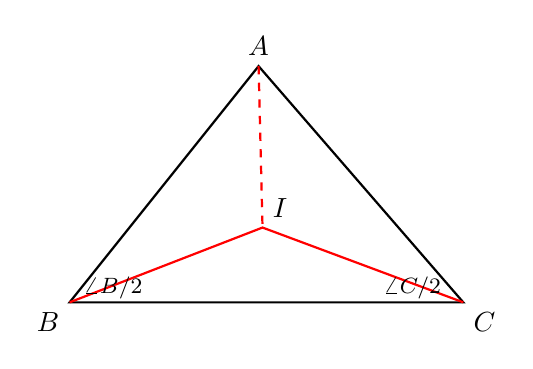
\begin{tikzpicture}[scale=1.0, thick]
  \coordinate (A) at (0, 3);
  \coordinate (B) at (-2.4, 0);
  \coordinate (C) at (2.6, 0);
  % I：近似为内心
  \coordinate (I) at (0.05, 0.95);

  \draw (A) -- (B) -- (C) -- cycle;
  \draw[red] (B) -- (I) -- (C);
  \draw[red, dashed] (A) -- (I);

  \node[above] at (A) {$A$};
  \node[below left] at (B) {$B$};
  \node[below right] at (C) {$C$};
  \node[above right] at (I) {$I$};

  % 标 BI, CI 是角平分线
  \node at ($(B)+(0.55, 0.18)$) {\footnotesize $\angle B/2$};
  \node at ($(C)+(-0.65, 0.18)$) {\footnotesize $\angle C/2$};
\end{tikzpicture}
\end{document}
